\chapter{DNA and Mutation System}
\label{ch:dna}

\epigraph{Nothing in biology makes sense except in the light of evolution.}{--- Theodosius Dobzhansky}

Every cancer cell is genetically unique, and this diversity determines which treatments succeed or fail. This chapter reveals how 16 key genes create tumor fingerprints --- and shows why males start with three times more cancer-driving mutations than females.

This chapter describes the gene-level representation used by tumor cells in the model.  The DNA system encodes 16 cancer-relevant genes, supports codon-level translation, introduces mutations during cell division with genomic-instability-dependent rates, and derives phenotypic parameters that govern tumor behavior and immune evasion.

%% ====================================================================
\section{Gene Model}
\label{sec:gene-model}

Each tumor cell carries a \texttt{DNA} object that encodes a synthetic DNA sequence containing 16 genes chosen for their relevance to renal cell carcinoma immunology.  The genes span the major biological axes of antigen presentation, immune checkpoint signaling, DNA repair, tumor suppression, and oncogenic proliferation.

\subsection{Gene Catalogue}

Table~\ref{tab:genes} lists all 16 genes, their functional categories, and their roles in the model.

\begin{longtable}{llp{7.5cm}}
\caption{The 16 genes modeled in the DNA system and their functional roles.}
\label{tab:genes} \\
\toprule
\textbf{Gene} & \textbf{Category} & \textbf{Functional Role} \\
\midrule
\endfirsthead
\toprule
\textbf{Gene} & \textbf{Category} & \textbf{Functional Role} \\
\midrule
\endhead
\midrule
\multicolumn{3}{r}{\textit{Continued on next page}} \\
\endfoot
\bottomrule
\endlastfoot
MHC    & Antigen Presentation   & Major histocompatibility complex; presents peptide antigens on the cell surface for T cell recognition. \\
B2M    & Antigen Presentation   & Beta-2-microglobulin; essential component of MHC class I molecules. \\
TAP1   & Antigen Presentation   & Transporter associated with antigen processing 1; loads peptides onto MHC I. \\
TAP2   & Antigen Presentation   & Transporter associated with antigen processing 2; works with TAP1 for peptide loading. \\
JAK1   & Antigen Presentation   & Janus kinase 1; IFN-$\gamma$ signaling for MHC upregulation. \\
JAK2   & Antigen Presentation   & Janus kinase 2; cooperates with JAK1 in interferon signaling. \\
CD274  & Immune Checkpoint      & PD-L1; binds PD-1 on T cells to induce immune checkpoint inhibition. \\
BRCA1  & DNA Repair             & Breast cancer type 1 susceptibility protein; key DNA double-strand break repair gene controlling genomic stability. \\
TP53   & Tumor Suppression      & Tumor protein p53; ``guardian of the genome,'' triggers apoptosis in damaged cells. \\
RB1    & Tumor Suppression      & Retinoblastoma protein; cell cycle checkpoint regulator. \\
CDKN2A & Tumor Suppression      & Cyclin-dependent kinase inhibitor 2A (p16); inhibits CDK4/6 to arrest cell cycle. \\
MYC    & Oncogene               & Transcription factor promoting cell growth and proliferation. \\
RAS    & Oncogene               & GTPase signal transducer in the MAPK proliferation pathway. \\
EGFR   & Oncogene               & Epidermal growth factor receptor; receptor tyrosine kinase driving proliferation. \\
HER2   & Oncogene               & Human epidermal growth factor receptor 2; amplified in aggressive tumors. \\
APC    & Tumor Suppression      & Adenomatous polyposis coli; Wnt pathway regulator, loss promotes proliferation. \\
\end{longtable}

\begin{figure}[htbp]
\centering
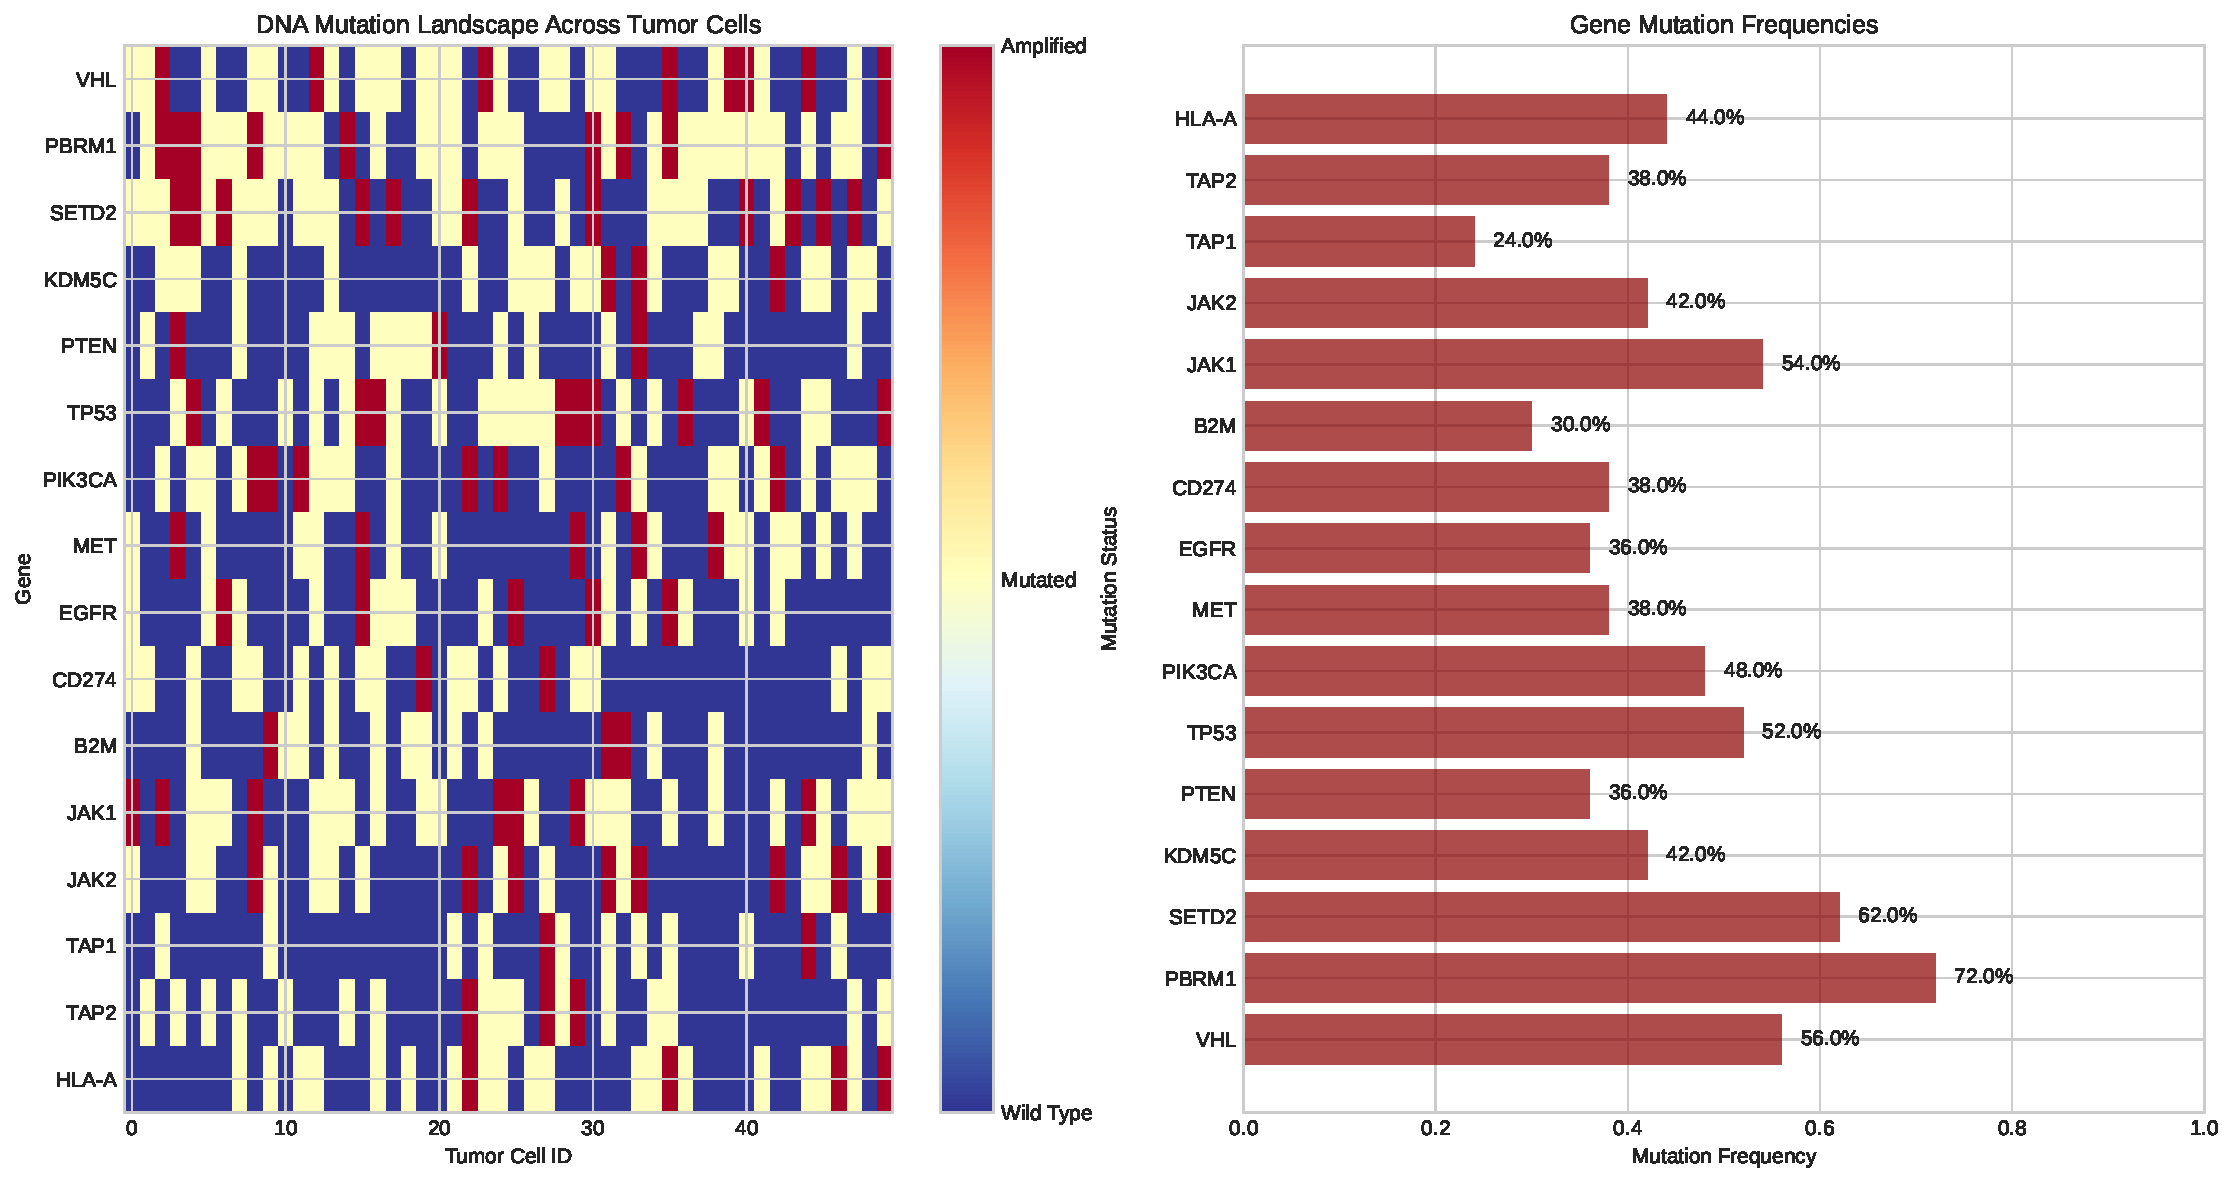
\includegraphics[width=0.85\textwidth]{figures/dna_mutation_heatmap.pdf}
\caption{DNA mutation heatmap across the 16 modeled genes showing the distribution of mutations in the tumor cell population. Each row represents a gene and each column represents a tumor cell lineage. Color intensity indicates the severity of mutation (darker colors represent higher mutation scores). The heterogeneous mutation patterns drive clonal diversity and immune evasion.}
\label{fig:dna_mutation_heatmap}
\end{figure}

\subsection{DNA Sequence Structure}

Each gene occupies a defined region within a synthetic DNA sequence.  The gene metadata specifies, for each gene: a start position (offset in the full DNA string), a coding region length of 90 base pairs, and a wildtype protein sequence of 20 amino acids.  The full DNA sequence is assembled during initialization by concatenating, for each gene:

\begin{enumerate}[nosep]
  \item A random nucleotide spacer (100~bp),
  \item A promoter region: 13 random bases, the \texttt{TATA} box motif, and 13 more random bases (total 30~bp),
  \item The coding region: codon-encoded wildtype protein (60~bp for 20 amino acids),
  \item A stop codon (\texttt{TAA}),
  \item A trailing spacer (7~bp).
\end{enumerate}

\noindent The start positions are fixed (at offsets 100, 300, 500, \ldots, 3100 for the 16 genes), ensuring deterministic gene location across all tumor cell lineages.  The wildtype protein sequences are fixed 20-character strings drawn from the standard amino acid alphabet.

%% ====================================================================
\section{Codon Translation}
\label{sec:codon-translation}

The model implements the standard genetic code, mapping all 64 possible nucleotide triplets to the 20 amino acids and the stop signal.

\subsection{Codon Table}

The codon table is stored as a class-level dictionary in the \texttt{DNA} class, with keys being three-letter nucleotide strings (e.g., \texttt{ATG} $\to$ \texttt{M} for methionine) and the three stop codons (\texttt{TAA}, \texttt{TAG}, \texttt{TGA}) mapping to the sentinel character \texttt{\_}.

\subsection{Translation: \texttt{gene\_to\_protein()}}

Given a gene name, the \texttt{gene\_to\_protein()} method reads codons starting from the gene's start position, translating each triplet to its corresponding amino acid.  Translation terminates upon encountering a stop codon:

\begin{lstlisting}[caption={Gene-to-protein translation.},label={lst:translation}]
def gene_to_protein(self, gene_name: str) -> str:
    protein = ""
    start = DNA.gene_metadata[gene_name]["start"]
    for i in range(start, len(self.dna) - 2, 3):
        codon = self.dna[i:i + 3]
        aa = self.codon_table.get(codon, 'X')
        if aa == '_':
            break
        protein += aa
    return protein
\end{lstlisting}

\noindent Unknown codons (which should not arise in practice) are mapped to \texttt{X}.

\subsection{Reverse Translation: \texttt{protein\_to\_gene()}}

For constructing the initial wildtype DNA sequence, the \texttt{protein\_to\_gene()} static method performs reverse translation.  It uses an inverted codon table (amino acid $\to$ codon) to convert each amino acid back to a nucleotide triplet.  Since the genetic code is degenerate (multiple codons per amino acid), the inverse mapping selects the last codon encountered during dictionary inversion, yielding a deterministic but arbitrary choice among synonymous codons.

%% ====================================================================
\section{Mutation Mechanics}
\label{sec:mutation-mechanics}

Mutations accumulate through two mechanisms: injected mutations at initialization and stochastic point mutations during DNA duplication.

\subsection{Genomic Instability}

The mutation rate during cell division is controlled by the genomic instability parameter, which is derived from the BRCA1 gene's mutation status:

\begin{equation}
\label{eq:genomic-instability}
\mu_{\text{instability}} = \bigl(s_{\text{BRCA1}}\bigr)^{\max(1,\; e_{\text{BRCA1}})} \times 0.05,
\end{equation}

\noindent where $s_{\text{BRCA1}}$ is the BRCA1 mutation score (see Section~\ref{sec:mutation-score}) and $e_{\text{BRCA1}}$ is the BRCA1 promoter expression level.  A wildtype BRCA1 ($s_{\text{BRCA1}} = 0$) yields zero instability, while a fully mutated BRCA1 ($s_{\text{BRCA1}} \to 1$) produces a base mutation rate of $0.05$ per nucleotide.  The exponentiation by the expression level amplifies the instability when the BRCA1 promoter is active.

\subsection{DNA Duplication with Point Mutations}

When a tumor cell divides, its DNA is duplicated with potential point mutations:

\begin{equation}
\label{eq:num-mutations}
n_{\text{mut}} = \lfloor \mu_{\text{instability}} \times L \rfloor,
\end{equation}

\noindent where $L$ is the total length of the DNA sequence.  For each of the $n_{\text{mut}}$ mutations, a random position is selected, and the nucleotide at that position is replaced by one of the three alternative bases (chosen uniformly at random).  This process models single-nucleotide variants (SNVs), the most common form of somatic mutation.

\subsection{Injected Mutations}

The initial cancer cell is seeded with pre-existing BRCA1 mutations to establish genomic instability from the outset.  The number of injected mutations depends on the patient's sex:

\begin{equation}
\label{eq:injected-mutations}
n_{\text{injected}} = \begin{cases} 3 & \text{if sex = Male,} \\ 1 & \text{if sex = Female.} \end{cases}
\end{equation}

\noindent These mutations are introduced by replacing a segment of the BRCA1 coding region (positions 730--790 in the DNA string) with a codon-encoded mutant protein that differs from the wildtype by exactly $n_{\text{injected}}$ amino acid substitutions.  The substitution positions are selected randomly, and each is replaced by a random alternative from the amino acid alphabet.

%% ====================================================================
\section{Gene Expression and Phenotypic Effects}
\label{sec:gene-expression}

\begin{figure}[htbp]
\centering
\adjustbox{max width=0.85\textwidth, max height=0.7\textheight}{% Tumor Cell State Machine Diagram
\begin{tikzpicture}[scale=0.9, every node/.style={scale=0.9}]

% Define states
\tikzstyle{state}=[draw, circle, minimum size=2cm, text width=1.8cm, text centered]
\tikzstyle{decision}=[draw, diamond, minimum size=1.5cm, text width=1.3cm, text centered, aspect=2]
\tikzstyle{action}=[draw, rectangle, rounded corners, minimum width=2cm, minimum height=1cm, text centered]

% States
\node[state, fill=tumorcell!20] (quiescent) at (0,0) {
    \textbf{Quiescent}\par
    Low metabolism\par
    Dormant
};

\node[state, fill=tumorcell!40] (active) at (6,0) {
    \textbf{Active}\par
    High glucose\par
    consumption
};

\node[state, fill=tumorcell!60] (dividing) at (12,0) {
    \textbf{Dividing}\par
    DNA replication\par
    Mitosis
};

\node[state, fill=tumorcell!80] (aggressive) at (6,-4) {
    \textbf{Aggressive}\par
    Angiogenesis\par
    Invasion
};

\node[state, fill=red!80] (apoptotic) at (0,-8) {
    \textbf{Apoptotic}\par
    Cell death\par
    pathway
};

% Decision points
\node[decision, fill=yellow!50] (growth_check) at (3,2) {
    Growth\par
    signals?
};

\node[decision, fill=yellow!50] (division_check) at (9,2) {
    Ready to\par
    divide?
};

\node[decision, fill=yellow!50] (stress_check) at (9,-2) {
    Stress\par
    signals?
};

\node[decision, fill=yellow!50] (immune_check) at (3,-6) {
    Immune\par
    attack?
};

% Actions
\node[action, fill=green!30] (consume_glucose) at (6,3) {
    Consume\par
    Glucose
};

\node[action, fill=green!30] (duplicate) at (12,3) {
    Create\par
    Daughter Cell
};

\node[action, fill=orange!30] (angiogenesis) at (9,-5) {
    Promote\par
    Angiogenesis
};

\node[action, fill=purple!30] (pd_l1) at (3,-3) {
    Express\par
    PD-L1
};

% Transitions with conditions
\draw[thick, ->] (quiescent) to[bend left=20] node[above] {\tiny Nutrients available} (growth_check);
\draw[thick, ->] (growth_check) -- node[right] {\tiny Yes} (active);
\draw[thick, ->] (growth_check) to[bend left=30] node[left] {\tiny No} (quiescent);

\draw[thick, ->] (active) -- (consume_glucose);
\draw[thick, ->] (consume_glucose) -- (active);

\draw[thick, ->] (active) -- node[above] {\tiny DNA replication complete} (division_check);
\draw[thick, ->] (division_check) -- node[right] {\tiny Yes} (duplicate);
\draw[thick, ->] (duplicate) -- (dividing);

\draw[thick, ->] (dividing) to[bend left=40] node[above] {\tiny Division complete} (active);

\draw[thick, ->] (division_check) to[bend left=20] node[left] {\tiny No} (active);

\draw[thick, ->] (active) to[bend right=20] node[right] {\tiny Hypoxia/stress} (stress_check);
\draw[thick, ->] (stress_check) -- node[right] {\tiny Yes} (aggressive);
\draw[thick, ->] (stress_check) to[bend right=20] node[below] {\tiny No} (active);

\draw[thick, ->] (aggressive) -- (angiogenesis);
\draw[thick, ->] (angiogenesis) -- (aggressive);

\draw[thick, ->] (aggressive) to[bend left=20] node[below] {\tiny Oxygen restored} (active);

% Immune evasion
\draw[thick, ->] (active) to[bend right=30] (pd_l1);
\draw[thick, ->] (aggressive) to[bend left=30] (pd_l1);
\draw[thick, ->] (pd_l1) to[bend right=20] (immune_check);

\draw[thick, ->] (immune_check) to[bend left=20] node[left] {\tiny Evaded} (active);
\draw[thick, ->] (immune_check) -- node[below] {\tiny Killed} (apoptotic);

% Death pathways
\draw[thick, ->, red] (quiescent) to[bend right=60] node[left] {\tiny DNA damage} (apoptotic);
\draw[thick, ->, red] (active) to[bend right=30] node[left] {\tiny Immune killing} (apoptotic);
\draw[thick, ->, red] (dividing) to[bend left=60] node[right] {\tiny Mitotic arrest} (apoptotic);
\draw[thick, ->, red] (aggressive) to[bend left=30] node[right] {\tiny Treatment} (apoptotic);

% Self loops for waiting states
\draw[thick, ->] (quiescent) to[loop above] node[above] {\tiny Wait} (quiescent);
\draw[thick, ->] (dividing) to[loop above] node[above] {\tiny Complete mitosis} (dividing);

% Title
\node[text width=14cm, text centered] at (6,6) {
    \Large\textbf{Tumor Cell State Machine and Decision Tree}
};

% Legend
\node[draw, rounded corners, fill=white, text width=3.5cm] at (-3,3) {
    \textbf{Legend}\par
    \textcolor{tumorcell}{\textbullet} Cellular States\par
    \textcolor{yellow!50}{\textbullet} Decision Points\par
    \textcolor{green!30}{\textbullet} Actions\par
    \textcolor{red}{—} Death Pathways
};

% Parameter influences
\node[draw, rounded corners, fill=blue!10, text width=4cm] at (15,1) {
    \textbf{Key Parameters}\par
    • \texttt{tumour\_growth\_effect}\par
    • \texttt{tumour\_apoptosis\_effect}\par
    • \texttt{angiogenesis\_effect}\par
    • DNA mutation profile\par
    • Glucose availability\par
    • Blood access
};

% DNA influence indicator
\node[draw, star, fill=dna, text=white] (dna) at (12,-2) {DNA};
\draw[thick, ->, dashed] (dna) -- (division_check) node[midway, right] {\tiny Mutation effects};
\draw[thick, ->, dashed] (dna) -- (pd_l1) node[midway, below] {\tiny CD274 expression};

\end{tikzpicture}}
\caption{State machine diagram of tumor cell lifecycle}
\label{fig:tumor_cell_state_machine}
\end{figure}

Each gene's contribution to tumor phenotype is determined by two quantities: promoter expression and mutation score.

\subsection{Promoter Expression}

Gene expression is modeled as a count of \texttt{TATA} motifs in the 30-nucleotide promoter region upstream of the coding sequence:

\begin{equation}
\label{eq:expression}
e_g = \#\{\texttt{TATA} \text{ occurrences in promoter region of gene } g\}.
\end{equation}

\noindent In the wildtype sequence, each gene has exactly one \texttt{TATA} box ($e_g = 1$).  Mutations in the promoter region can destroy or create additional \texttt{TATA} motifs, thereby altering expression.

\subsection{Mutation Score}
\label{sec:mutation-score}

The mutation score quantifies how far the translated protein has diverged from the wildtype:

\begin{equation}
\label{eq:mutation-score}
s_g = 1 - \text{Levenshtein.ratio}\bigl(p_g^{\text{wt}},\; p_g^{\text{mut}}\bigr),
\end{equation}

\noindent where $p_g^{\text{wt}}$ is the wildtype protein sequence, $p_g^{\text{mut}}$ is the mutant protein, and $\text{Levenshtein.ratio}$ returns the normalized similarity (1.0 for identical strings, 0.0 for completely different strings).  A mutation score of $s_g = 0$ indicates a wildtype protein, while $s_g = 1$ indicates maximal divergence.

\subsection{Gene Mutation--Expression Product}

Several phenotypic parameters use the product of expression and mutation score:

\begin{equation}
\label{eq:gene-mut-expr}
\phi_g = e_g \cdot s_g,
\end{equation}

\noindent which captures the idea that a gene must be both expressed and mutated to exert a phenotypic effect.

\subsection{Five Derived Phenotypic Parameters}

The DNA system computes five aggregate phenotypic parameters from the 16 individual gene states.  These parameters directly influence tumor cell behavior during simulation.

\paragraph{1.\ Antigen Presentation Chance.}
\begin{equation}
\label{eq:antigen-presentation}
p_{\text{AP}} = \max\!\left(0,\; 6 - \frac{\sum_{g \in \mathcal{G}_{\text{AP}}} \phi_g}{6}\right),
\end{equation}
where $\mathcal{G}_{\text{AP}} = \{\text{MHC, JAK1, JAK2, B2M, TAP1, TAP2}\}$.  This represents the tumor cell's ability to present antigens on its surface.  Mutations in antigen presentation genes reduce this probability, enabling immune evasion.

\begin{tcolorbox}[enhanced, colback=blue!3, colframe=blue!50!black, arc=3pt, boxrule=0.5pt, title={\textbf{Key Takeaway}}]
Males start with three times more BRCA1 mutations than females, creating higher genomic instability from the very beginning. Each tumor cell carries a unique 16-gene fingerprint that determines its visibility to the immune system, growth rate, and treatment response.
\end{tcolorbox}

\paragraph{2.\ Checkpoint Pathway Inhibition Chance.}
\begin{equation}
\label{eq:checkpoint}
p_{\text{CPI}} = \phi_{\text{CD274}},
\end{equation}
determined solely by the CD274 (PD-L1) gene.  Higher expression of mutated PD-L1 increases the probability that the tumor cell will engage the PD-1 checkpoint on interacting T cells, suppressing their cytotoxic activity.

\paragraph{3.\ Genomic Instability.}
\begin{equation}
\label{eq:genomic-instability-param}
\mu_{\text{instability}} = \bigl(s_{\text{BRCA1}}\bigr)^{\max(1,\; e_{\text{BRCA1}})} \times 0.05,
\end{equation}
as described in Section~\ref{sec:mutation-mechanics}.  This parameter controls the mutation rate during DNA duplication.

\paragraph{4.\ Tumor Suppression Chance.}
\begin{equation}
\label{eq:tumor-suppression}
p_{\text{TS}} = \frac{1}{3}\sum_{g \in \mathcal{G}_{\text{TS}}} e_g \cdot (1 - s_g),
\end{equation}
where $\mathcal{G}_{\text{TS}} = \{\text{TP53, RB1, CDKN2A}\}$.  Functional (unmutated, expressed) tumor suppressors increase the probability of apoptosis.  Loss-of-function mutations ($s_g \to 1$) diminish this protective effect.

\paragraph{5.\ Extra Proliferation Chance.}
\begin{equation}
\label{eq:extra-proliferation}
p_{\text{EP}} = \frac{1}{5}\left(\sum_{g \in \mathcal{G}_{\text{onco}}} e_g \cdot (1 - s_g) + \phi_{\text{APC}}\right),
\end{equation}
where $\mathcal{G}_{\text{onco}} = \{\text{MYC, RAS, EGFR, HER2}\}$.  This parameter captures oncogene-driven proliferation.  Functional oncogenes and mutated APC (a tumor suppressor whose loss promotes proliferation via the Wnt pathway) both contribute to increased growth.  The raw value is converted to a probability using a saturating transformation:
\begin{equation}
\label{eq:gene-expr-to-chance}
\hat{p}_{\text{EP}} = 1 - e^{-k \cdot p_{\text{EP}}}, \qquad k = 0.01.
\end{equation}

%% ====================================================================
\section{Neoantigen Generation}
\label{sec:neoantigens}

The mutation system provides the molecular basis for adaptive immune recognition of tumor cells.

\subsection{Neoantigen Definition}

Neoantigens are short peptide fragments derived from mutated proteins.  In the model, neoantigens are represented as 10-mer subsequences (10 consecutive amino acids) extracted from each translated protein:

\begin{equation}
\label{eq:neoantigens}
\mathcal{N} = \bigcup_{g \in \mathcal{G}} \bigl\{ p_g^{\text{mut}}[i:i{+}10] \;\big|\; 0 \leq i \leq 9 \bigr\},
\end{equation}

\noindent where $p_g^{\text{mut}}$ is the mutated protein sequence for gene $g$ and the set union is taken over all 16 genes.

\subsection{Self-Antigens}

The set of self-antigens is computed from the wildtype protein sequences using the same 10-mer extraction:

\begin{equation}
\label{eq:self-antigens}
\mathcal{S} = \bigcup_{g \in \mathcal{G}} \bigl\{ p_g^{\text{wt}}[i:i{+}10] \;\big|\; 0 \leq i \leq |p_g^{\text{wt}}| - 10 \bigr\}.
\end{equation}

\noindent Self-antigens are computed once (as a class-level cached set) since the wildtype sequences are identical across all cells.

\subsection{TCR Matching}

T cell receptors (TCRs) recognize neoantigens through a matching mechanism based on Hamming distance:

\begin{enumerate}[nosep]
  \item The 10-mer antigen peptide is hashed to an 8-bit value using SHA-256 (taking the first byte of the digest).
  \item The T cell's receptor is a random 8-bit integer generated at initialization.
  \item The Hamming distance (number of differing bits) between the antigen hash and the receptor is computed.
  \item A match is declared if the antigen is \emph{not} a self-antigen and the Hamming distance is within a threshold:
\end{enumerate}

\begin{equation}
\label{eq:tcr-matching}
\text{match}(a, r) = \bigl(a \notin \mathcal{S}\bigr) \;\wedge\; \bigl(d_H\bigl(h(a),\, r\bigr) \leq 3 + \Delta_r\bigr),
\end{equation}

\noindent where $h(a)$ is the 8-bit hash of antigen $a$, $r$ is the receptor value, $d_H$ denotes Hamming distance, and $\Delta_r$ is the \texttt{receptor\_threshold\_variation} parameter (default $1$, giving a threshold of $4$).  This mechanism ensures that T cells only respond to foreign (non-self) peptides and provides a stochastic, receptor-specific recognition model.

These genetic mutations create vulnerabilities that treatments can exploit. The next chapter examines exactly how immune checkpoint inhibitors and targeted therapies turn cancer's own molecular weaknesses against itself.
